\documentclass[10pt]{article}

\def\Type{LessonCaelan}
\def\TypeNum{Lesson 11}
\def\TypeTitle{Local Extrema \& First Derivative Test \\Solutions}
\def\Semester{Fall 2021} %Not Used 
\def\Course{MATH 1190 \& 1210}
\def\Targets{ {\bf\color{RedOrange}A1}, {\bf\color{RedOrange}A2} }

\usepackage{preambleDJ}

%\usepackage{ragged2e}


%%%%%%%%%%%% BEGIN DOCUMENT %%%%%%%%%%%%%%%
%%%%%%%%%%%% BEGIN DOCUMENT %%%%%%%%%%%%%%%
%%%%%%%%%%%% BEGIN DOCUMENT %%%%%%%%%%%%%%%
%%%%%%%%%%%% BEGIN DOCUMENT %%%%%%%%%%%%%%%
%%%%%%%%%%%% BEGIN DOCUMENT %%%%%%%%%%%%%%%



\begin{document}

\pagestyle{otherpages}
\thispagestyle{firstpage}
\vs{.8}

\textbf{Intended Learning Outcomes}
After this lesson, you will be able to 

\begin{itemize}
    \item Identify increasing/decreasing intervals and critical numbers of a function from given graph or formula. (\target{A1})
    \item Represent concepts such as derivatives, local extrema, and critical number graphically. (\target{A1})
    \item Apply the First Derivative Test to determine the local extrema of a function graphically and algebraically. (\target{A2})
\end{itemize}

\vspace{-0.5cm}

\hrulefill\\
In this activity, we establish a means of finding local extreme values (also called relative extreme values) of a function using properties of the derivative. First, review some key ideas from the online class prep activity to prepare yourself for the important ideas of the lesson.\\

{\bf \textcolor{blue}{Warm-up Exercise 1.}}\ltrm{\color{RedOrange}A1}  Respond to the prompt below.
%
 \important{Definition: Critical Number}
    {
    A {\em critical number} is  a number $c$ in the \blue{\it domain} of $f$ where either
  \begin{center} \blue{ $f'(c) = 0$} \quad\quad\quad or \quad\quad\quad \blue{$f'(c) \qquad DNE$} \end{center}
    }
    
    {\bf TRUE or FALSE?} $\displaystyle f(x)=\frac1x$ has exactly 1 critical number. \hfill (circle one): \hfill {\bf TRUE} \hfill {\bf FALSE}\\ Explain your decision.
    \sol{False. $f'(x)=-x^{-2}=-\dfrac{1}{x^2}$, so $f'(x)=0$ has no solution and $f'(x)$ DNE when $x=0$. However $f(0)$ is not defined, so $x=0$ is not a critical number of $f(x)$.}
 \\\\
{\bf \color{blue} Mini-lecture: } Connecting the sign of $f'$ to the locations of local extrema.\\
\mpageT{.33}{.8}[\hs{.1}]{
%
\includegraphics[width=0.95\textwidth]{images/1st derivative test.PNG}
\begin{flushleft}
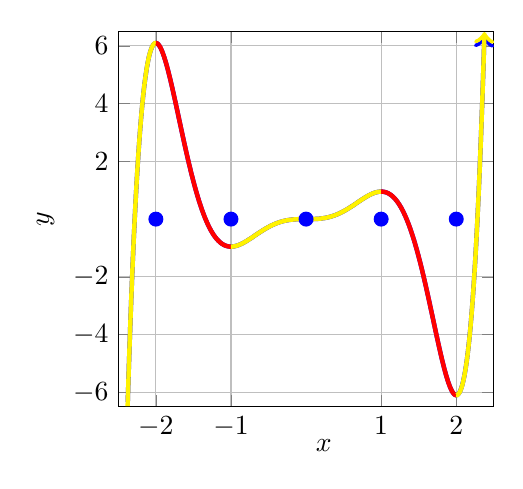
\begin{tikzpicture}
    \begin{axis}[
    	x label style={anchor=west},
            xlabel={$x$},
            xtick       = {-2,-1,1,2},
            xticklabels = {$-2$,$-1$,$1$,$2$},
            y label style={anchor=south},
            ylabel={$y$},
            ytick       = {-6,-4,-2,2,4,6},
            yticklabels = {$-6$,$-4$,$-2$,$2$,$4$,$6$},
            samples     = 320,
            domain      = -2.5:2.5,
            restrict y to domain=-6.5:6.5,
            xmin = -2.5, xmax = 2.5,
            ymin = -6.5, ymax = 6.5,
            width=2.5in, height=2.5in,
            grid=both, grid style=solid
          ]
    \addplot[domain=-2.5:2.5, blue, ultra thick, mark=none, ->]{2*(x^7/7-x^5+4/3*x^3)};
        \addplot[domain=-2.5:-2, yellow, ultra thick, mark=none, -]{2*(x^7/7-x^5+4/3*x^3)};
                \addplot[domain=-2:-1, red, ultra thick, mark=none, -]{2*(x^7/7-x^5+4/3*x^3)};
                                \addplot[domain=-1:1, yellow, ultra thick, mark=none, -]{2*(x^7/7-x^5+4/3*x^3)};
                                                \addplot[domain=1:2, red, ultra thick, mark=none, -]{2*(x^7/7-x^5+4/3*x^3)};
                                                                                \addplot[domain=2:2.5, yellow, ultra thick, mark=none, ->]{2*(x^7/7-x^5+4/3*x^3)};
            \filldraw[blue] (-2,0) circle (2.5pt);
\filldraw[blue] (-1,0) circle (2.5pt);
\filldraw[blue] (0,0) circle (2.5pt);
\filldraw[blue] (1,0) circle (2.5pt);
\filldraw[blue] (2,0) circle (2.5pt);
    \end{axis}
\end{tikzpicture}
\end{flushleft}
\itemNIN{
\item Highlight  graph where increasing. \blue{(See yellow portions of graph)}
\item Highlight  graph where decreasing.  \blue{(See red portions of graph)}
\item Place a point on the graph at each critical number.  \blue{(See blue points on $x$-axis.)}
}
}{
 \important{First Derivative Test}
	{
	Suppose that $c$ is a \blue{\em critical number} of a continuous function $f$.
			\enumA{
			\mpageT{.6}{.4}{
			\item If $f'$ changes from \blue{(+)} to \blue{(-)} at $c$, then $f$ has:\\
			\blue{Local maximum. This occurs at $x=-2,1$.}\vs{.3}
			}{
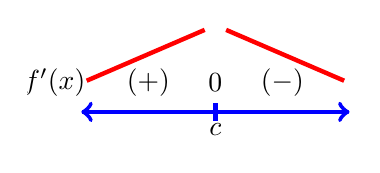
\begin{tikzpicture}
    \begin{axis}[
    	axis x line=none,
	            axis y line=none,
		x label style={anchor=west},
            xlabel={},
            xtick       = {0},
            xticklabels = {$c$},
            y label style={anchor=south},
            ylabel={},
            ytick       = {-6,-4,-2,2,4,6},
            yticklabels = {$-6$,$-4$,$-2$,$2$,$4$,$6$},
            samples     = 320,
            domain      = -2.5:2.5,
            restrict y to domain=-6.5:6.5,
            xmin = -3.5, xmax = 3.5,
            ymin = -6.5, ymax = 6.5,
            width=2.5in, height=2.5in,
            grid=none, grid style=solid
          ]
    \addplot[domain=-2.5:2.5, blue, ultra thick, mark=none, <->]{0)};
   \draw (-3,1) node{$\Large f^{\prime}(x)$};
   \draw[ultra thick, blue] (0,.3)--(0,-.3);
      \draw (0,-.6) node{$c$};
            \draw (0,1) node{$0$};
            \addplot[domain=-2.4:-.2, red, ultra thick, mark=none, -]{2*x/2.5+3)};
                        \addplot[domain=0.2:2.4, red, ultra thick, mark=none, -]{-2*x/2.5+3)};
                             \draw (-1.25,1) node{\blue{$(+)$}};
                              \draw (1.25,1) node{\blue{$(-)$}};
    \end{axis}
\end{tikzpicture}
			}
			\mpageT{.6}{.4}{
			\item If $f'$ changes from \blue{(-)} to \blue{(+)} at $c$, then $f$ has:\\
			\blue{Local minimum. This occurs at $x=-1,2$.}\vs{.3}
			}{
			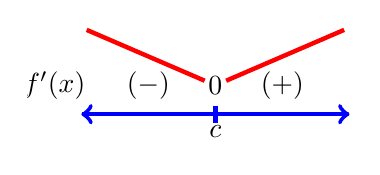
\begin{tikzpicture}
    \begin{axis}[
    	axis x line=none,
	            axis y line=none,
		x label style={anchor=west},
            xlabel={},
            xtick       = {0},
            xticklabels = {$c$},
            y label style={anchor=south},
            ylabel={},
            ytick       = {-6,-4,-2,2,4,6},
            yticklabels = {$-6$,$-4$,$-2$,$2$,$4$,$6$},
            samples     = 320,
            domain      = -2.5:2.5,
            restrict y to domain=-6.5:6.5,
            xmin = -3.5, xmax = 3.5,
            ymin = -6.5, ymax = 6.5,
            width=2.5in, height=2.5in,
            grid=none, grid style=solid
          ]
    \addplot[domain=-2.5:2.5, blue, ultra thick, mark=none, <->]{0)};
   \draw (-3,1) node{$\Large f^{\prime}(x)$};
   \draw[ultra thick, blue] (0,.3)--(0,-.3);
      \draw (0,-.6) node{$c$};
        \draw (0,1) node{$0$};
            \addplot[domain=-2.4:-.2, red, ultra thick, mark=none, -]{-2*x/2.5+1)};
                        \addplot[domain=0.2:2.4, red, ultra thick, mark=none, -]{2*x/2.5+1)};
                             \draw (-1.25,1) node{\blue{$(-)$}};
                              \draw (1.25,1) node{\blue{$(+)$}};
    \end{axis}
\end{tikzpicture}
}
\mpageT{.6}{.4}{
			\item If $f'$ does not change sign at $c$, then $f$ has:\\
				\blue{Neither local maximum nor minimum. This occurs at $x=-0$.}\vs{.3}
			}{
			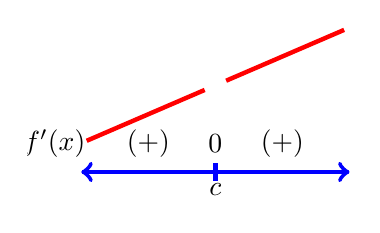
\begin{tikzpicture}
    \begin{axis}[
    	axis x line=none,
	            axis y line=none,
		x label style={anchor=west},
            xlabel={},
            xtick       = {0},
            xticklabels = {$c$},
            y label style={anchor=south},
            ylabel={},
            ytick       = {-6,-4,-2,2,4,6},
            yticklabels = {$-6$,$-4$,$-2$,$2$,$4$,$6$},
            samples     = 320,
            domain      = -2.5:2.5,
            restrict y to domain=-6.5:6.5,
            xmin = -3.5, xmax = 3.5,
            ymin = -6.5, ymax = 6.5,
            width=2.5in, height=2.5in,
            grid=none, grid style=solid
          ]
    \addplot[domain=-2.5:2.5, blue, ultra thick, mark=none, <->]{0)};
   \draw (-3,1) node{$\Large f^{\prime}(x)$};
   \draw[ultra thick, blue] (0,.3)--(0,-.3);
      \draw (0,-.6) node{$c$};
       \draw (0,1) node{$0$};
            \addplot[domain=-2.4:-.2, red, ultra thick, mark=none, -]{2*x/2.5+3)};
                        \addplot[domain=0.2:2.4, red, ultra thick, mark=none, -]{2*x/2.5+3)};
                             \draw (-1.25,1) node{\blue{$(+)$}};
                              \draw (1.25,1) node{\blue{$(+)$}};
    \end{axis}
\end{tikzpicture}
}
			}
	}
}

\newpage
 
 {\bf \textcolor{blue}{Warm-up Exercise 2}} \ltrm{\target{A1}}  Sketch the graph of a function $f$ satisfying the following:\\
 
\begin{minipage}[t]{0.6\textwidth}
 \begin{itemize}
 \item $f'(2)=0$ and $f(2)$ is a local/relative minimum
 \item $f'(4)=0$ and $f(4)$ is neither a maximum nor a minimum
 \item $f'(6)$ DNE and $f(6)$ is a local/relative maximum
 \end{itemize}
 \vs{-.2}
 \sol{
 There are many  graphs that  satisfy these $3$ criteria.  
 \itemI{
 \item At $x=2$, we have a local minimum. The tangent line (in blue) has slope of $0$ and thus $f^{\prime}(2)=0$
 \item At $x=4$, the tangent line (in blue) has slope of $0$ and thus $f^{\prime}(4)=0$
 \item At $x=6$ we have a peak (i.e. a local max) but since this is a corner, $f^{\prime}(6)$ DNE
 }
 }
 \end{minipage}
 \hfill
 \begin{minipage}[t]{0.38\textwidth}
 \vspace{-0.2in}
 \begin{center}
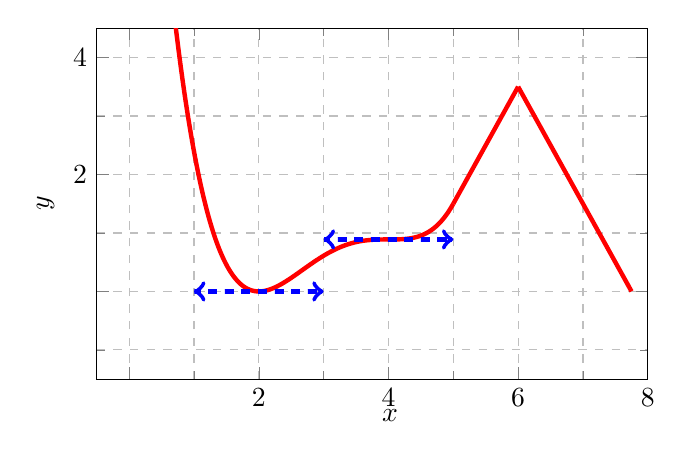
\begin{tikzpicture}
    \begin{axis}[scale=2.,
    	x label style={anchor=west},
            xlabel={$x$},
            xtick       = {0,2,4,6,8},
            xticklabels = {,$2$,$4$,$6$,$8$},
            y label style={anchor=south},
            ylabel={$y$},
            ytick       = {-2,0,2,4},
            yticklabels = {,,$2$,$4$},
            minor tick num=1,
            samples     = 320,
            domain      = -.5:8,
            restrict y to domain=0:5,
            xmin = -.5, xmax = 8,
            ymin = -1.5, ymax = 4.5,
            width=2in, height=1.5in,
            grid=both, grid style=dashed
          ]
    \addplot[domain=0:5, red, ultra thick, mark=none, -]{1/18*(x-2)^2*(3*x^2-28*x+68)};
        \addplot[dashed, domain=1:3, blue, ultra  thick, mark=none, <->]{0};
        \addplot[domain=5:6, red, ultra thick, mark=none, -]{2*x-17/2};
                \addplot[dashed, domain=3:5, blue, ultra  thick, mark=none, <->]{8/9};
                \addplot[domain=6:8, red, ultra thick, mark=none, -]{-2*x+31/2};
    \end{axis}
\end{tikzpicture}
 \end{center}
 \end{minipage}
 


\example Let $g(x)=x-\ln(x^2+1)$.
%
\begin{enumerate}
\item[(a)]\ltrm{\target{A1}} Find the critical numbers of $g$.


\sol{$g'(x)=1-\dfrac{1}{x^2+1}\cdot 2x=1-\dfrac{2x}{x^2+1}=\dfrac{x^2-2x+1}{x^2+1}=\dfrac{(x-1)^2}{x^2+1}$

If $g'(x)=0$, we get $(x-1)^2=1$, or $x=1$.

If $g'(x)$ DNE, we get $x^2+1=0$, which has no solution.

$g(1)=1-\ln(2)$ is defined, so $g(x)$ is continuous at $x=1$, which means $x=1$ is a critical number of $g(x)$.}
\\

\item[(b)]\ltrm{\color{RedOrange}\bf A1} Find the intervals where $g$ is increasing or decreasing. {\em Hint:} Creating a sign line will probably be helpful.

\sol{We can make a sign line to record the sign of $g'(x)$. The critical number $x=1$ splits the number line into two intervals. For each interval, we can plug in a value to determine the sign of $g'(x)$ on this interval.

$g'(0)=1-0=1>0$

$g'(2)=1-\dfrac{2\cdot 2}{2^2+1}=\dfrac{1}{5}>0$

\begin{center}
\begin{tikzpicture}[scale=1]
              \begin{axis}[
              axis y line=left,
            xlabel={$x$},
            ylabel={},
            xlabel style={anchor=west},
	  y axis line style={draw=none},
	  	  x axis line style={draw opacity=0},
            %grid = major,
            every major tick/.append style={ thick, blue, major tick length=5pt},
            xtick       = {  1},
            xticklabels = { $1$ },
            ytick       = \empty,
            yticklabels={},
                                      y  axis line style=-,
                          % y axis/.append style={y axis line style=-}
            samples     = 320,
            restrict y to domain=-40:40,
            xmin = -2, xmax = 3,
            ymin = -.5, ymax = 1.5,
            height=1.5in, width=2.75in
          ]
	\draw[thick,<->] (-1,0) -- (3,0);
	 \node[anchor=west] at (-1.5,.5) {\small $g^{\prime}(x)$};
	  	   \node at (1,.5) {\small $0$};
	    %\node at (-.8,.5) {\small $0$};
		\node at (0,.5) {\small $(+)$};
		\node at (2,.5) {\small $(+)$};
		%\draw[ultra thick, red] (-.8,1.5) -- (-.05,.8);
		%\draw[ultra thick, red] (.05,.8) -- (.8,1.5);
          %
        \end{axis}
    \end{tikzpicture}
\end{center}

Since $g'(x)$ is positive on the intervals $(-\infty, 1)$ and $(1, \infty)$, we get $g(x)$ is increasing on the intervals $(-\infty, 1)$ and $(1, \infty)$. $g(x)$ is never decreasing.

Note: We can't say $g(x)$ is increasing on $(-\infty, \infty)$ because $g(x)$ is not increasing at $x=1$.
}


\item[(c)]\ltrm{\color{RedOrange}\bf A2} At which critical number(s) does $g$ attain a local extreme value(s)? Explicitly cite a relevant test in your response.

\sol{The sign of $g'(x)$ does not change at its critical number $x=1$, so by the First Derivative Test, $g(x)$ has neither a local maximum nor a local minimum at $x=1$.}

\end{enumerate}

\newpage

\exercise Let $f(x)=\dfrac{x}{x^2+1}$.
\begin{enumerate}
\item[(a)] \ltrm{\color{RedOrange}\bf A1} Find the intervals where $f$ is increasing or decreasing. Draw a number line to depict your answer, and record your final answer using interval notation. \\

\sol{$f'(x)=\dfrac{(x^2+1)-x(2x)}{(x^2+1)^2}=\dfrac{1-x^2}{(x^2+1)^2}$

If $f'(x)=0$, we get $1-x^2=0$, or $x=\pm 1$.

If $f'(x)$ DNE, we get $(x^2+1)^2=0$, which has no solution.

Both $f(-1)=\dfrac{-1}{1+1}=-\dfrac{1}{2}$ and $f(1)=\dfrac{1}{1+1}=\dfrac{1}{2}$ are defined, so both $x=-1$ and $x=1$ are critical numbers of $f(x)$.

These two critical numbers split the number line into three parts. For each part, we plug in a number to determine the sign of $f'(x)$ on it.

$f'(-2)=\dfrac{1-4}{4+1}=-\dfrac{3}{5}<0$

$f'(0)=\dfrac{1-0}{0+1}=1>0$

$f'(2)=\dfrac{1-4}{4+1}=-\dfrac{3}{5}<0$

\begin{center}
\begin{tikzpicture}[scale=1]
              \begin{axis}[
              axis y line=left,
            xlabel={$x$},
            ylabel={},
            xlabel style={anchor=west},
	  y axis line style={draw=none},
	  	  x axis line style={draw opacity=0},
            %grid = major,
            every major tick/.append style={ thick, blue, major tick length=5pt},
            xtick       = { -1, 1},
            xticklabels = { $-1$, $1$ },
            ytick       = \empty,
            yticklabels={},
                                      y  axis line style=-,
                          % y axis/.append style={y axis line style=-}
            samples     = 320,
            restrict y to domain=-40:40,
            xmin = -4, xmax = 3,
            ymin = -.5, ymax = 1.5,
            height=1.5in, width=2.75in
          ]
	\draw[thick,<->] (-3,0) -- (3,0);
	 \node[anchor=west] at (-4,.5) {\small $f^{\prime}(x)$};
	  	\node at (1,.5) {\small $0$};
	    \node at (-1,.5) {\small $0$};
		\node at (0,.5) {\small $(+)$};
        \node at (-2,.5) {\small $(-)$};
		\node at (2,.5) {\small $(-)$};
		%\draw[ultra thick, red] (-.8,1.5) -- (-.05,.8);
		%\draw[ultra thick, red] (.05,.8) -- (.8,1.5);
          %
        \end{axis}
    \end{tikzpicture}
\end{center}

Therefore, $f(x)$ is increasing on the interval $(-1, 1)$, and $f(x)$ is decreasing on the intervals $(-\infty, -1)$ and $(1, \infty)$.

}



\item[(b)] \ltrm{\color{RedOrange}\bf A2} Find the local maximum \& local minimum points of $f$. Explicitly cite a relevant test in your response. \\

\sol{$f'(x)$ changes from negative to positive at $x=-1$, so by the First Derivative Test, $f(x)$ has a local minimum at $x=-1$.

$f'(x)$ changes from positive to negative at $x=1$, so by the First Derivative Test, $f(x)$ has a local maximum at $x=-1$.}
\end{enumerate}

\newpage
{\bf Note:} The next problem will test your conceptual understanding of what it means for a function to increase or decrease, as well as of the definition of a critical number. A variation of this problem appeared on an exam during the Fall 2023 semester.\\
\exercise{{\bf\color{RedOrange}A1}}  What would the {\em critical numbers} of the function $f$ be if...
\enumA{
\mpageT{.55}{.45}{
\vs{.3}
%\enumA{
\item  the curve pictured to the right is the graph of $f$? 
\sol{
 $x=2,4,6$\\
We can see that $f$ has horizontal tangent lines at $x=2, 4, 6$, which means $f'(x)=0$ at them. $f$ is clearly defined at these three points, so these three points are critical numbers of $f$. In addition, $f$ is a smooth curve with no corners, vertical tangents, nor discontinuities, so $f$ has no additional critical numbers.
}
%}
}{
\begin{flushright}
    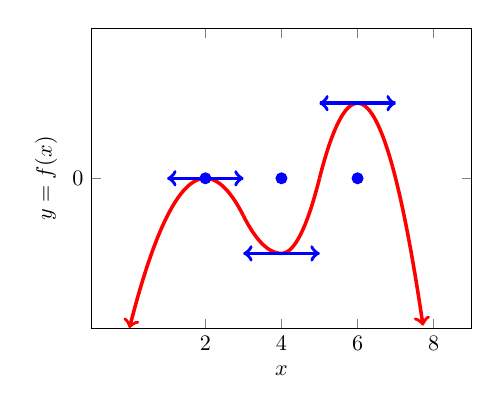
\begin{tikzpicture}[scale=.8]
          \begin{axis}[
            xlabel={$x$},
            ylabel={$y=f(x)$},
            %grid = major,
            xtick       = {2,4,6,8},
            xticklabels = {$2$,$4$,$6$,$8$},
            ytick       = {0},
            yticklabels = {$0$},
            samples     = 320,
            domain      = -1:9,
            restrict y to domain=-4:4,
            xmin = -1, xmax = 9,
            ymin = -4, ymax = 4,
            height=2.5in, width=3in
          ]
%
          \addplot[domain=-1:3, ultra thick, red,<-] {-(x-2)^2};
          \addplot[domain=3:4, ultra thick, red] {(x-4)^2-2};
          \addplot[domain=4:5, ultra thick, red] {2*(x-4)^2-2};
          \addplot[domain=5:9, ultra thick, red,->] {-2*(x-6)^2+2};
          \addplot[domain=1:3, blue, ultra  thick, mark=none, <->]{0};
           \addplot[domain=3:5, blue, ultra  thick, mark=none, <->]{-2};
            \addplot[domain=5:7, blue, ultra  thick, mark=none, <->]{2};
            \filldraw[blue] (2,0) circle (2.5pt);
            \filldraw[blue] (4,0) circle (2.5pt);
            \filldraw[blue] (6,0) circle (2.5pt);
          %
        \end{axis}
    \end{tikzpicture}
\end{flushright}
}

\mpageT{.55}{.45}{\vs{.3}
%\enumA{\setItemnumber{2}
\item the curve pictured to the right is the graph of $f'$? 
\sol{
$x=2,5,7$\\
This is the graph of $f^{\prime}(x)$.  $f^{\prime}(x)=0$ when the  $y-$value is $0$.  This occurs at $x= 2, 5, 7$, so these are the points where $f'(x)=0$, which means they are critical numbers of $f$. Since $f'$ is defined everywhere in the graph, $f$ has no additional critical numbers.
}
%}
}{
\begin{flushright}
    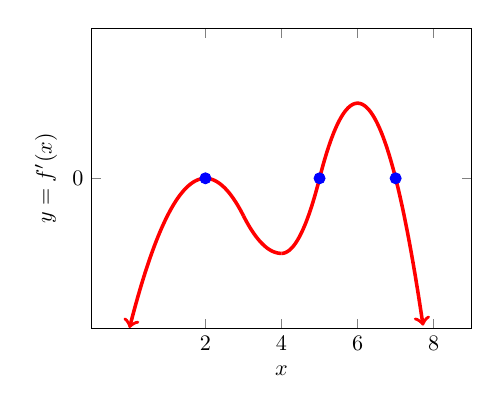
\begin{tikzpicture}[scale=.8]
          \begin{axis}[
            xlabel={$x$},
            ylabel={$y=f^{\prime}(x)$},
            %grid = major,
            xtick       = {2,4,6,8},
            xticklabels = {$2$,$4$,$6$,$8$},
            ytick       = {0},
            yticklabels = {$0$},
            samples     = 320,
            domain      = -1:9,
            restrict y to domain=-4:4,
            xmin = -1, xmax = 9,
            ymin = -4, ymax = 4,
            height=2.5in, width=3in
          ]
%
	\addplot[domain=-1:3, ultra thick, red,<-] {-(x-2)^2};
	\addplot[domain=3:4, ultra thick, red] {(x-4)^2-2};
	\addplot[domain=4:5, ultra thick, red] {2*(x-4)^2-2};
	\addplot[domain=5:9, ultra thick, red,->] {-2*(x-6)^2+2};
	\filldraw[blue] (2,0) circle (2.5pt);
	\filldraw[blue] (5,0) circle (2.5pt);
	\filldraw[blue] (7,0) circle (2.5pt);
          %
        \end{axis}
    \end{tikzpicture}
\end{flushright}
}
}
\exercise{{\bf\color{RedOrange}A1}}  On which intervals would the function $f$ be {\it decreasing} if...
\enumA{
\mpageT{.55}{.45}{
\item the curve pictured to the right is the graph of $f$?
\sol{
$f$ is decreasing when $f^{\prime}(x)<0$.  We see the graph trending down  on $(2, 4)$ and $(6, \infty)$. We do {\em not} include $x=2$, $x=4$ nor $x=6$ since $f^{\prime}(x)=0$ at those points.
}
}{
\begin{flushright}
    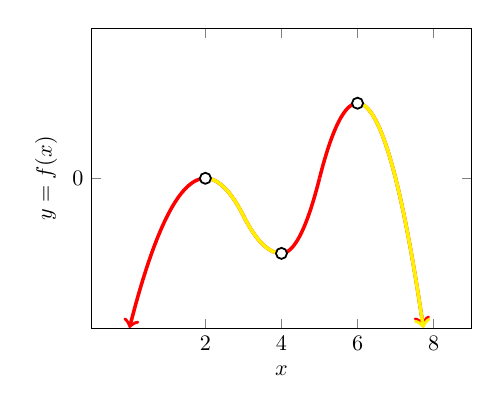
\begin{tikzpicture}[scale=.8]
          \begin{axis}[
            xlabel={$x$},
            ylabel={$y=f(x)$},
            %grid = major,
            xtick       = {2,4,6,8},
            xticklabels = {$2$,$4$,$6$,$8$},
            ytick       = {0},
            yticklabels = {$0$},
            samples     = 320,
            domain      = -1:9,
            restrict y to domain=-4:4,
            xmin = -1, xmax = 9,
            ymin = -4, ymax = 4,
            height=2.5in, width=3in
          ]
          % old version of the curve
          %
          %\addplot[domain=-1:9, purple, ultra thick, mark=none] {-1/10*(x-1)*(x-4)^2*(x-7)};
          %
          %new version of the curve in pieces
          %
	\addplot[domain=-1:3, ultra thick, red,<-] {-(x-2)^2};
	\addplot[domain=3:4, ultra thick, red] {(x-4)^2-2};
	\addplot[domain=4:5, ultra thick, red] {2*(x-4)^2-2};
	\addplot[domain=5:9, ultra thick, red,->] {-2*(x-6)^2+2};
	\addplot[domain=2:3, ultra thick, yellow] {-(x-2)^2};
	\addplot[domain=3:4, ultra thick, yellow] {(x-4)^2-2};
	\filldraw[white] (2,0) circle (2.5pt);
	\draw[thick] (2,0) circle (2.5pt);
	\filldraw[white] (4,-2) circle (2.5pt);
	\draw[thick] (4,-2) circle (2.5pt);
	\addplot[domain=6:9, ultra thick, yellow,->] {-2*(x-6)^2+2};
	\filldraw[white] (6,2) circle (2.5pt);
	\draw[thick] (6,2) circle (2.5pt);
          %
        \end{axis}
    \end{tikzpicture}
\end{flushright}
}
\mpageT{.55}{.45}{
\vs{.3}
\item the curve pictured to the right is the graph of $f'$?
\sol{
$f(x)$ (not pictured on the right) is decreasing when $f^{\prime}(x)<0$. Since we are given a graph of $y=f^{\prime}(x)$  it is negative when the $y$-values are negative. This occurs on the intervals $(-\infty, 2)$, $(2, 5)$, and $(7, \infty)$, so $f$ is decreasing on these intervals.
}
}{
\begin{flushright}
    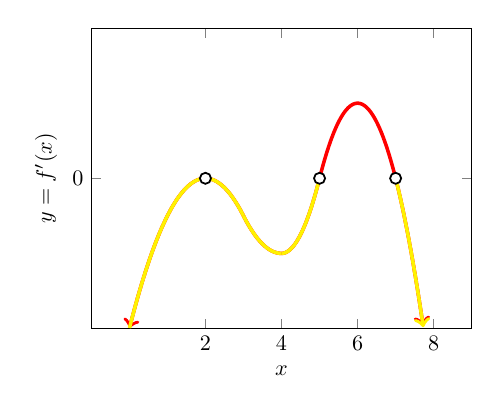
\begin{tikzpicture}[scale=.8]
          \begin{axis}[
            xlabel={$x$},
            ylabel={$y=f^{\prime}(x)$},
            %grid = major,
            xtick       = {2,4,6,8},
            xticklabels = {$2$,$4$,$6$,$8$},
            ytick       = {0},
            yticklabels = {$0$},
            samples     = 320,
            domain      = -1:9,
            restrict y to domain=-4:4,
            xmin = -1, xmax = 9,
            ymin = -4, ymax = 4,
            height=2.5in, width=3in
          ]
%
	\addplot[domain=-1:3, ultra thick, red,<-] {-(x-2)^2};
	\addplot[domain=3:4, ultra thick, red] {(x-4)^2-2};
	\addplot[domain=4:5, ultra thick, red] {2*(x-4)^2-2};
	\addplot[domain=5:9, ultra thick, red,->] {-2*(x-6)^2+2};
	\addplot[domain=-1:3, ultra thick, yellow] {-(x-2)^2};
	\addplot[domain=3:4, ultra thick, yellow] {(x-4)^2-2};
          \addplot[domain=4:5, ultra thick, yellow] {2*(x-4)^2-2};
	\addplot[domain=7:9, ultra thick, yellow,->] {-2*(x-6)^2+2};
          %
	\filldraw[white] (2,0) circle (2.5pt);
	\draw[thick] (2,0) circle (2.5pt);
	\filldraw[white] (5,0) circle (2.5pt);
	\draw[thick] (5,0) circle (2.5pt);
	\filldraw[white] (7,0) circle (2.5pt);
	\draw[thick] (7,0) circle (2.5pt);
          %
        \end{axis}
    \end{tikzpicture}
\end{flushright}
}
}




\newpage
{\bf Note:} The next problem will test your comprehension of Warm-up Exercise 1 and the Chain Rule.\\

{\bf\color{blue} Extra Practice 1.}\ltrm{\color{RedOrange}A1} Find all critical numbers of $f(x)=\sqrt[3]{x^2-4x}$.

\sol{
$f(x)=(x^2-4x)^{1/3}$

$f'(x)=\dfrac{1}{3}(x^2-4x)^{-2/3}(2x-4)=\dfrac{2x}{3(x^2-4x)^{2/3}}$

If $f'(x)=0$, we get $2x-4=0$, or $x=2$.

If $f'(x)$ DNE, we get $x^2-4x=0$, or $x(x-4)=0$. This gives $x=0$ and $x=4$.

The domain of $f$ is all real numbers, so $f$ is defined at $x=0, 2, 4$, which means these three numbers are the critical numbers of $f$.

}

\vs{.5}


{\bf Note:} The next 2 exercises make use of all the information in this worksheet and the associated pre-class assignment. The goal is for you to continue to fluently apply the definition of a critical number, to find \& interpret the sign of the first derivative as it relates to whether a function is increasing or decreasing, and to use the First Derivative Test to classify critical numbers.\\

{\bf\color{blue} Extra Practice 2.} Let $f(x)=\ln(x^2-2x+1)$. 
\enumA{
\item \ltrm{\color{RedOrange}A1} Find all critical numbers of $f$.
    
\sol{
$f'(x)=\dfrac{2x-2}{x^2-2x+1}=\dfrac{2(x-1)}{(x-1)^2}=\dfrac{2}{x-1}$

If $f'(x)=0$, we get $2=0$, which is impossible.

If $f'(x)$ DNE, we get $x-1=0$, or $x=1$.

$f(1)=\ln(1-2+1)=\ln(0)$, which is undefined. So $f(x)$ has no critical number.

}
    
\item \ltrm{\color{RedOrange}A1} Find the intervals on which $f$ is increasing \& the intervals on which $f$ is decreasing.

\sol{

Even if $x=1$ is not a critical number, it is a point where $f'(x)$ DNE, so we still use it to split the number line into two parts.

$f'(0)=\dfrac{2}{0-1}=-2<0$

$f'(2)=\dfrac{2}{2-1}=2>0$

\begin{center}
\begin{tikzpicture}[scale=1]
              \begin{axis}[
              axis y line=left,
            xlabel={$x$},
            ylabel={},
            xlabel style={anchor=west},
	  y axis line style={draw=none},
	  	  x axis line style={draw opacity=0},
            %grid = major,
            every major tick/.append style={ thick, blue, major tick length=5pt},
            xtick       = {  1},
            xticklabels = { $1$ },
            ytick       = \empty,
            yticklabels={},
                                      y  axis line style=-,
                          % y axis/.append style={y axis line style=-}
            samples     = 320,
            restrict y to domain=-40:40,
            xmin = -2, xmax = 3,
            ymin = -.5, ymax = 1.5,
            height=1.5in, width=2.75in
          ]
	\draw[thick,<->] (-1,0) -- (3,0);
	 \node[anchor=west] at (-1.5,.5) {\small $f^{\prime}(x)$};
	  	   \node at (1,.5) {\small $DNE$};
	    %\node at (-.8,.5) {\small $0$};
		\node at (0,.5) {\small $(-)$};
		\node at (2,.5) {\small $(+)$};
		%\draw[ultra thick, red] (-.8,1.5) -- (-.05,.8);
		%\draw[ultra thick, red] (.05,.8) -- (.8,1.5);
          %
        \end{axis}
    \end{tikzpicture}
\end{center}

Therefore, $f(x)$ is increasing on the interval $(1, \infty)$, and $f(x)$ is decreasing on the interval $(-\infty, 1)$.

}


\item \ltrm{\color{RedOrange}A2} At which $x$-values does $f$ have local maximum values? At which $x$-values does $f$ have local minimum values? Explain.
\sol{

$f$ has no local extrema since $f$ has no critical number.

}
}

%%%%%%%%%
\newpage%
%%%%%%%%%

{\bf\color{blue} Extra Practice 3.} Let $f(x)=\dfrac15x^5-\dfrac53x^3+4x$.
\enumA{
\item \ltrm{\color{RedOrange}A1} Find the critical numbers of $f$.
\sol{

$f'(x)=x^4-5x^2+4=(x^2-4)(x^2-1)=(x-2)(x+2)(x-1)(x+1)$

If $f'(x)=0$, we get $x=-2, -1, 1, 2$.

There's no $x$-values for which $f'(x)$ DNE, since $f'(x)$ is a polynomial defined for all real numbers.

So the critical numbers of $f(x)$ are $x=-2, -1, 1, 2$.

}
\item \ltrm{\color{RedOrange}A1} Find the intervals where $f$ is increasing or decreasing.
\sol{

The critical numbers split the number line into five intervals: $(-\infty, -2)$, $(-2, -1)$, $(-1, 1)$, $(1, 2)$, and $(2, \infty)$.

\begin{table}[h!]
    \centering
    \blue{
    \begin{tabular}{c|cccc|c}
      $x$  & $x+2$ & $x+1$ & $x-1$ & $x-2$ & $f'(x)$\\
      \hline
        $(-\infty, -2)$ & - & - & - & - & +\\
        $(-2, -1)$ & + & - & - & - & -\\
        $(-1, 1)$ & + & + & - & - & +\\
        $(1, 2)$ & + & + & + & - & -\\
        $(2, \infty)$ & + & + & + & + & +\\
    \end{tabular}
    }
\end{table}

Therefore, $f(x)$ is increasing on the intervals $(-\infty, -2)$, $(-1, 1)$, $(2, \infty)$, and $f(x)$ is decreasing on the intervals $(-2, -1)$ and $(1, 2)$.

}  

\item \ltrm{\color{RedOrange}A2} At which critical number(s) does $f$ attain local extrema? Explain.
\sol{

At $x=-2$ and $x=1$, $f'(x)$ changes from positive to negative, so by the First Derivative Test, $f$ has local maxima at these critical numbers.

At $x=-1$ and $x=2$, $f'(x)$ changes from negative to positive, so by the First Derivative Test, $f$ has local minima at these critical numbers.
}
}
\newpage
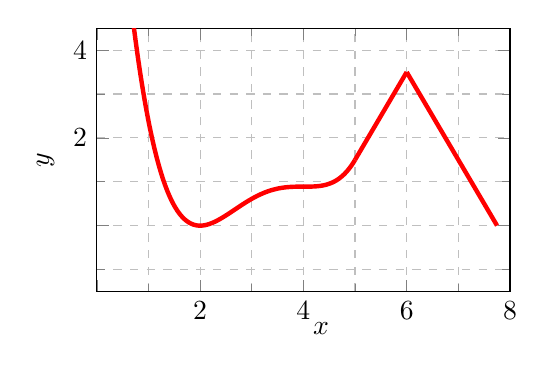
\begin{tikzpicture}
    \begin{axis}[scale=1.5,
    	x label style={anchor=west},
            xlabel={$x$},
            xtick       = {0,2,4,6,8},
            xticklabels = {,$2$,$4$,$6$,$8$},
            y label style={anchor=south},
            ylabel={$y$},
            ytick       = {-2,0,2,4},
            yticklabels = {,,$2$,$4$},
            minor tick num=1,
            samples     = 320,
            domain      = -.5:8,
            restrict y to domain=0:5,
            xmin = 0, xmax = 8,
            ymin = -1.5, ymax = 4.5,
            width=2in, height=1.5in,
            grid=both, grid style=dashed
          ]
    \addplot[domain=0:5, red, ultra thick, mark=none, -]{1/18*(x-2)^2*(3*x^2-28*x+68)};
        \addplot[domain=5:6, red, ultra thick, mark=none, -]{2*x-17/2};
                \addplot[domain=6:8, red, ultra thick, mark=none, -]{-2*x+31/2};
    \end{axis}
\end{tikzpicture}


\end{document}


\end{document}
